%%%% ijcai18.tex

\typeout{IJCAI-18 Instructions for Authors}

% These are the instructions for authors for IJCAI-18.
% They are the same as the ones for IJCAI-11 with superficical wording
%   changes only.

\documentclass{article}
\pdfpagewidth=8.5in
\pdfpageheight=11in
% The file ijcai18.sty is the style file for IJCAI-18 (same as ijcai08.sty).
\usepackage{ijcai18}

% Use the postscript times font!
\usepackage{times}
\usepackage{xcolor}
\usepackage{soul}
\usepackage[utf8]{inputenc}
\usepackage[small]{caption}

\usepackage{amsmath}
\usepackage{amssymb}
\usepackage{amsthm}
\usepackage{multirow}
\usepackage{tikz}
\usepackage{comment}

\newcommand{\tup}[1]{{\langle #1 \rangle}}

\newcommand{\pre}{\mathsf{pre}}     % precondition
\newcommand{\del}{\mathsf{del}}     % effect
\newcommand{\add}{\mathsf{add}}     % effect
\newcommand{\eff}{\mathsf{eff}}     % effect
\newcommand{\cond}{\mathsf{cond}}   % conditional effect
\newcommand{\true}{\mathsf{true}}   % true
\newcommand{\false}{\mathsf{false}} % false
\newcommand{\PE}{\mathrm{PE}}     % precondition
\newcommand{\strips}{\textsc{Strips}}     % strips

\newtheorem{theorem}{Theorem}
\newtheorem{lemma}[theorem]{Lemma}
\newtheorem{definition}[theorem]{Definition}

\usepackage{graphicx}
\usepackage{caption}
\usepackage{subcaption}
\usepackage{listings}
\usepackage{multicol}
\usepackage{arydshln}
\usetikzlibrary{calc,backgrounds,positioning,fit}

% the following package is optional:
%\usepackage{latexsym} 

% Following comment is from ijcai97-submit.tex:
% The preparation of these files was supported by Schlumberger Palo Alto
% Research, AT\&T Bell Laboratories, and Morgan Kaufmann Publishers.
% Shirley Jowell, of Morgan Kaufmann Publishers, and Peter F.
% Patel-Schneider, of AT\&T Bell Laboratories collaborated on their
% preparation.

% These instructions can be modified and used in other conferences as long
% as credit to the authors and supporting agencies is retained, this notice
% is not changed, and further modification or reuse is not restricted.
% Neither Shirley Jowell nor Peter F. Patel-Schneider can be listed as
% contacts for providing assistance without their prior permission.

% To use for other conferences, change references to files and the
% conference appropriate and use other authors, contacts, publishers, and
% organizations.
% Also change the deadline and address for returning papers and the length and
% page charge instructions.
% Put where the files are available in the appropriate places.

\title{Learning \strips\ Action Models from State-Constraints}

\author{Diego Aineto\and Sergio Jim\'enez\and Eva Onaindia\\
{\small Departamento de Sistemas Inform\'aticos y Computaci\'on}\\
{\small Universitat Polit\`ecnica de Val\`encia.}\\
{\small Camino de Vera s/n. 46022 Valencia, Spain}\\
{\small \{dieaigar,serjice,onaindia\}@dsic.upv.es}}

\begin{document}

\maketitle

\begin{abstract}
This paper presents a classical planning compilation for learning \strips\ action models from state-constraints. The compilation approach does not require observations of the precise executed actions because an off-the-shelf classical planner leverages on the given constraints to determine the executed actions. In addition the paper introduces a novel evaluation method to asses the learning of \strips\ models even when actions are {\em reformulated} because the learning task is too low-constrained. 
\end{abstract}

\section{Introduction}
Besides {\em plan synthesis}~\cite{ghallab2004automated}, planning action models are also useful for {\em plan/goal recognition}~\cite{ramirez2012plan}. At these planning tasks, automated planners are required to reason about an action model that correctly and completely captures the possible world transitions~\cite{geffner:book:2013}. Unfortunately, building planning action models is complex, even for planning experts, and this knowledge acquisition task is a bottleneck that limits the potential of {\em AI planning}~\cite{kambhampati:modellite:AAAI2007}.

The Machine Learning of planning action models is a promising alternative to hand-coding them and nowadays, there exist sophisticated algorithms like {\sc ARMS}~\cite{yang2007learning}, {\sc SLAF}~\cite{amir:alearning:JAIR08} or {\sc LOCM}~\cite{cresswell2013acquiring}. Motivated by recent advances on the synthesis of different kinds of generative models with classical planning~\cite{bonet2009automatic,segovia2016hierarchical,segovia2017generating}, this paper introduces an innovative approach for learning \strips\ action models that:
\begin{enumerate}
\item Is defined as a classical planning compilation, which opens the door to the {\em bootstrapping} of planning action models.
\item Does not require observations of the particular executed actions. An off-the-shelf classical planner leverages on the given constraints to determine the executed actions.
\item Can assess the learned \strips\ models with respect to a {\em reference model}, even when learning is so low constrained that actions are reformulated and still compliant with the learning inputs. 
\end{enumerate}
 

\section{Background}
This section defines the planning models used in this work as well as the input (the state constraints) and output (an \strips\ action model) of the addressed learning task.

\subsection{Classical planning}
We use $F$ to denote the set of {\em fluents} (propositional variables) describing a state. A {\em literal} $l$ is a valuation of a fluent $f\in F$, i.e. either~$l=f$ or $l=\neg f$. A set of literals $L$ represents a partial assignment of values to fluents (WLOG we assume that $L$ does not assign conflicting values to any fluent). We use $\mathcal{L}(F)$ to denote the set of all literal sets on $F$, i.e.~all partial assignments of values to fluents.

A {\em state} $s$ is a full assignment of values to fluents, i.e. $|s|=|F|$, so the size of the state space is $2^{|F|}$. Explicitly including negative literals $\neg f$ in states simplifies subsequent definitions but often, we will abuse notation by defining a state $s$ only in terms of the fluents that are true in $s$, as is common in \strips\ planning.

A {\em classical planning frame} is a tuple $\Phi=\tup{F,A}$, where $F$ is a set of fluents and $A$ is a set of actions. Each action $a\in A$ comprises three sets of literals:
\begin{itemize}
\item $\pre(a)\subseteq\mathcal{L}(F)$, called {\em preconditions}, the literals that must hold for the action $a\in A$ to be applicable.
\item $\eff^+(a)\subseteq\mathcal{L}(F)$, called {\em positive effects}, that defines the fluents set to true by the application of the action $a\in A$.
\item $\eff^-(a)\subseteq\mathcal{L}(F)$, called {\em negative effects}, that defines the fluents set to false by the action application.
\end{itemize}
We say that an action $a\in A$ is {\em applicable} in a state $s$ iff $\pre(a)\subseteq s$. The result of applying $a$ in $s$ is the {\em successor state} denoted by $\theta(s,a)=\{s\setminus\eff^-(a))\cup\eff^+(a)\}$.

A {\em classical planning problem} is a tuple $P=\tup{F,A,I,G}$, where $I$ is an initial state and $G\subseteq\mathcal{L}(F)$ is a goal condition. A {\em plan} for $P$ is an action sequence $\pi=\tup{a_1, \ldots, a_n}$ that induces the {\em state trajectory} $\tup{s_0, s_1, \ldots, s_n}$ such that $s_0=I$ and, for each {\small $1\leq i\leq n$}, $a_i$ is applicable in $s_{i-1}$ and generates the successor state $s_i=\theta(s_{i-1},a_i)$. The {\em plan length} is denoted with $|\pi|=n$ . A plan $\pi$ {\em solves} $P$ iff $G\subseteq s_n$, i.e.~if the goal condition is satisfied at the last state reached after following the application of the plan $\pi$ in the initial state $I$.


\subsection{Classical planning with conditional effects}
Our approach for learning \strips\ action models is compiling the leaning task into a classical planning task with conditional effects. Conditional effects allow us to compactly define actions whose effects depend on the current state. Supporting conditional effects is now a requirement of the {\em International Planning Competition}~\cite{vallati:IPC:AIM2015} and many classical planners cope with conditional effects without compiling them away.

An action $a\in A$ is now defined as a set of {\em preconditions} $\pre(a)\in\mathcal{L}(F)$ and a set of {\em conditional effects} $\cond(a)$. Each conditional effect $C\rhd E\in\cond(a)$ is composed of two sets of literals $C\in\mathcal{L}(F)$, the {\em condition}, and $E\in\mathcal{L}(F)$, the {\em effect}. An action $a\in A$ is {\em applicable} in a state $s$ if and only if $\pre(a)\subseteq s$, and the {\em triggered effects} resulting from the action application are the effects whose conditions hold in $s$:
\[
triggered(s,a)=\bigcup_{C\rhd E\in\cond(a),C\subseteq s} E,
\]
The result of applying an action $a$ in a state $s$ is the {\em successor} state $\theta(s,a)=\{s\setminus\eff_c^-(s,a))\cup\eff_c^+(s,a)\}$ where $\eff_c^-(s,a)\subseteq triggered(s,a)$ are the triggered {\em negative} effects and $\eff_c^+(s,a)\subseteq triggered(s,a)$ are the triggered {\em positive} effects.


\subsection{State-constraints}
The notion of state-constraint is very general and has been used in different areas of AI and for different purposes.  If we restrict ourselves to planning, {\em state-constraints} are abstractions for compactly specifying sets of states. For instance to specify the states where a given action is applicable or that are considered goal states.  A particular kind of state-constraints useful for planning is {\em invariants}. {\em State invariant} are traditionally used for computing more compact state representations~\cite{helmert2009concise} and/or for making {\em satisfiability planning} and {\em backward search} more efficient~\cite{rintanen2014madagascar,alcazar2015reminder}.

Given a classical planning problem $P=\tup{F,A,I,G}$, a {\em state invariant} is a formula $\phi$ that holds at the initial state of a given classical planning problem, $I\models \phi$, and at every state $s$ that is reachable from $I$. The formula $\phi_{I,A}^*$ represents the {\em strongest invariant} and exactly characterizes the set of all states reachable from $I$ using the actions in $A$. A {\em mutex} (mutually exclusive) is a state invariant that takes the form of a binary clause and indicates a pair of different properties that cannot be simultaneously true~\cite{kautz:mutex:IJCAI1999}. For instance in a three-blocks {\em blocksworld}, $\phi_1=\neg on(block_1,block_2)\vee \neg on(block_1,block_3)$ are mutex because $block_1$ can only be on top of a single block. 

A {\em domain invariant} is an instance-independent state invariant, i.e. holds for any possible initial state. Domain invariants are often compactly defined as {\em lifted invariant} (also called schematic invariant) that is state invariants defined as a first order formula~\cite{rintanen:schematicInvariants:AAAI2017}. For instance in the {\em blocksworld}, $\phi_2=\forall x:\ (\neg handempty\vee \neg holding(x))$, is a {\em domain mutex} because the robot hand is never empty and holding a block at the same time. In this work we exploit {\em domain invariants} to constrain the possible \strips\ action models and reduce then the learning hypothesis space.

\begin{figure}
\begin{scriptsize}
\begin{verbatim}
(:action stack
 :parameters (?v1 ?v2 - object)
 :precondition (and (holding ?v1) (clear ?v2))
  :effect (and (not (holding ?v1)) (not (clear ?v2))
               (handempty) (clear ?v1) (on ?v1 ?v2)))
\end{verbatim}
\end{scriptsize}
 \caption{\small \strips\ operator schema coding, in PDDL, the {\em stack} action from the {\em blocksworld}.}
\label{fig:stack}
\end{figure}

\subsection{\strips\ action schemes}
This work addresses the learning of PDDL action schemes that follow the \strips\ requirement~\cite{mcdermott1998pddl,fox2003pddl2}. Figure~\ref{fig:stack} shows the {\em stack} action schema, coded in PDDL, from a four-operator {\em blocksworld}~\cite{slaney2001blocks}.

To formalize the output of the learning task, we assume that fluents $F$ are instantiated from a set of {\em predicates} $\Psi$, as in PDDL. Each predicate $p\in\Psi$ has an argument list of arity $ar(p)$. Given a set of {\em objects} $\Omega$, the set of fluents $F$ is induced by assigning objects in $\Omega$ to the arguments of predicates in $\Psi$, i.e.~$F=\{p(\omega):p\in\Psi,\omega\in\Omega^{ar(p)}\}$ s.t. $\Omega^k$ is the $k$-th Cartesian power of $\Omega$.

Let $\Omega_v=\{v_i\}_{i=1}^{\operatorname*{max}_{a\in A} ar(a)}$ be a new set of objects ($\Omega\cap\Omega_v=\emptyset$), denoted as {\em variable names}, and that is bound by the maximum arity of an action in a given planning frame. For instance, in a three-block blocksworld $\Omega=\{block_1, block_2, block_3\}$ while $\Omega_v=\{v_1, v_2\}$ because the operators with the maximum arity, {\small\tt stack} and {\small\tt unstack}, have two parameters.

Let us also define $F_v$, a new set of fluents $F\cap F_v=\emptyset$, that results from instantiating $\Psi$ using only the objects in $\Omega_v$ and that defines the elements that can appear in an action schema. For instance, in the blocksworld, $F_v$={\small\tt\{handempty, holding($v_1$), holding($v_2$), clear($v_1$), clear($v_2$), ontable($v_1$), ontable($v_2$), on($v_1,v_1$), on($v_1,v_2$), on($v_2,v_1$), on($v_2,v_2$)\}}.

Finally, we assume that actions $a\in A$ are instantiated from \strips\ operator schemes $\xi=\tup{head(\xi),pre(\xi),add(\xi),del(\xi)}$ where:
\begin{itemize}
\item $head(\xi)=\tup{name(\xi),pars(\xi)}$, is the operator {\em header} defined by its name and corresponding {\em variable names}, $pars(\xi)=\{v_i\}_{i=1}^{ar(\xi)}$. For instance, the headers for a four-operator blocksworld are: {\small\tt pickup($v_1$), putdown($v_1$), stack($v_1,v_2$)} and {\small\tt unstack($v_1,v_2$)}.
\item The preconditions $pre(\xi)\subseteq F_v$, the negative effects $del(\xi)\subseteq F_v$, and the positive effects $add(\xi)\subseteq F_v$ such that, $del(\xi)\subseteq pre(\xi)$, $del(\xi)\cap add(\xi)=\emptyset$ and $pre(\xi)\cap add(\xi)=\emptyset$.
\end{itemize}


\section{Learning \strips\ action models}
Learning \strips\ action models from fully available input knowledge, i.e. from plans where every action in the plan is available as well as its corresponding {\em pre-} and {\em post-states}, is straightforward. %In this case, \strips\ operator schemes are derived lifting the literals that change between the pre and post-state of the corresponding action executions. Preconditions are derived lifting the minimal set of literals that appears in all the pre-states of the corresponding actions.

We formalize a more challenging learning task, where less input knowledge is available. This learning task corresponds to observing an agent acting in the world but watching only the results of its plan executions, the actual executed actions are unobserved. Formally the addressed learning task is defined as $\Lambda=\tup{\Psi,\Sigma,\Phi}$:
\begin{itemize}
\item $\Psi$ is the set of predicates that define the abstract state space of a given classical planning frame.
\item $\Sigma=\{\sigma_1,\ldots,\sigma_{\tau}\}$ is a set of $(initial, final)$ state pairs, that we call {\em labels}. Each label $\sigma_t=(s_0^t,s_{n}^t)$, {\tt\small $1\leq t\leq \tau$}, comprises the {\em final} state $s_{n}^t$ resulting from executing an unobserved plan $\pi_t$ starting from the {\em initial} state $s_0^t$.
\item $\Phi$ is a set of {\em domain invariants}, note that they do not necessary contain the {\em strongest invariant}.
\end{itemize}

A solution to $\Lambda$ is a set of operator schema $\Xi$ compliant with the predicates in $\Psi$, the labels $\Sigma$, and the state-constraints $\Phi$. A planning compilation is a suitable approach for addressing $\Lambda$ learning task because a solution must not only determine the \strips\ action model $\Xi$ but also, the {\em unobserved} plans $\pi_t=\tup{a_1^t, \ldots, a_n^t}$, {\tt\small $1\leq t\leq \tau$} that can explain $\Sigma$ and $\Phi$. Figure~\ref{fig:lexample} shows an example of a $\Lambda$ task for learning a \strips\ action model in the blocksworld from a single label $\sigma_1$ and a set of nine state invariants.

\begin{figure}
{\footnotesize\tt ;;; Predicates in $\Psi$}
\begin{scriptsize}
\begin{verbatim}
(handempty) (holding ?o  - object)
(clear ?o - object) (ontable ?o - object)
(on ?o1 - object ?o2 - object)
\end{verbatim}
\end{scriptsize}
\vspace{0.2cm}
\begin{subfigure}{.6\textwidth}
{\footnotesize\tt ;;; Label $\sigma_1=(s_0^1,s_{n}^1)$}
\begin{lstlisting}[mathescape]
\end{lstlisting}
\vspace{-0.2cm}
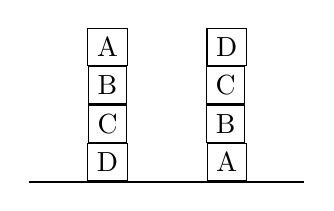
\begin{tikzpicture}[node distance = 0mm, block/.style args = {#1,#2}{fill=#1,text width=#2,shape=square}]
\node (initD) [draw]{D};
\node (initC) [draw, above=of initD.north]{C};
\node (initB) [draw, above=of initC.north]{B};
\node (initA) [draw, above=of initB.north]{A};
\draw[thick] (-1,-0.25) -- (2.5,-0.25);

\node (goalA) [draw, right=10mm of initD]{A};
\node (goalB) [draw, right=10mm of initC]{B};
\node (goalC) [draw, right=10mm of initB]{C};
\node (goalD) [draw, right=10mm of initA]{D};
\end{tikzpicture}
\end{subfigure}%
\vspace{0.6cm}
\begin{subfigure}{.6\textwidth}
{\footnotesize\tt ;;; Lifted domain invariants in $\Phi$}
\begin{scriptsize}
\begin{verbatim}
 (forall (?o1 - object)
   (not (and (on ?o1 ?o1))))

 (forall (?o1 - object)
   (not (and (handempty) (holding ?o1)))))

 (forall (?o1 - object)
   (not (and (holding ?o1) (clear ?o1)))))

 (forall (?o1 - object)
   (not (and (holding ?o1) (ontable ?o1))))

 (forall (?o1 ?o2 - object)
   (not (and (on ?o1 ?o2) (holding ?o1))))

 (forall (?o1 ?o2 - object)
   (not (and (on ?o1 ?o2) (holding ?o2))))

 (forall (?o1 ?o2 - object)
    (not (and (on ?o1 ?o2) (clear ?o2))))

 (forall (?o1 ?o2 - object)
    (not (and (on ?o1 ?o2) (ontable ?o1))))

 (forall (?o1 ?o2 - object)
    (not (and (on ?o1 ?o2) (on ?o2 ?o1)))))
\end{verbatim}
\end{scriptsize}
\end{subfigure}%
 \caption{\small Example of a task for learning a \strips\ action model in the blocksworld from a single label and nine state-invariants.}
\label{fig:lexample}
\end{figure}

\subsection{Learning with classical planning}

Our approach for addressing the learning task $\Lambda$, is compiling it into a classical planning task with conditional effects. The intuition behind the compilation is that a solution to the resulting classical planning task is a sequence of actions that:
\begin{enumerate}
\item Programs the \strips\ action model $\Xi$. A solution plan starts with a {\em prefix} that, for each $\xi\in\Xi$, determines which fluents $f\in F_v$ belong to its $pre(\xi)$, $del(\xi)$ and $add(\xi)$ sets.
\item Validates the programmed \strips\ action model $\Xi$ in $\Sigma$ and $\Phi$. A solution plan continues with, for every $\sigma_t\in \Sigma$, a postfix that produces a final state $s_{n}^t$ starting from the corresponding initial state $s_0^t$ using the programmed action model $\Xi$ and satisfying the constraints $\phi\in\Phi$ at every reached state. We call this process the validation of the programmed \strips\ action model $\Xi$, at the $t^{th}$ learning example, {\small $1\leq t\leq \tau$}. %If information about the corresponding plan $\pi_t\in \Pi$ is available, then it is also used in the validation.
\end{enumerate}

To formalize our compilation we first define {\small $1\leq t\leq \tau$} classical planning instances $P_t=\tup{F,\emptyset,I_t,G_t}$ that belong to the same planning frame (same fluents and actions but different initial state and/or goals). Fluents $F$ are built instantiating the predicates in $\Psi$ with the objects appearing in the input labels $\Sigma$. Formally $\Omega=\{o|o\in \bigcup_{\small 1\leq t\leq \tau} obj(s_0^t)\}$, where $obj$ is a function that returns the set of objects that appear in a fully specified state. The set of actions, $A=\emptyset$, is empty because the action model is initially unknown. Finally, the initial state $I_t$ is given by the state $s_0^t\in \sigma_t$ while goals $G_t$, are defined by the state $s_n^t\in \sigma_t$.

Now we are ready to formalize the compilation. Given a learning task $\Lambda=\tup{\Psi,\Sigma,\Phi}$ the compilation outputs a classical planning task $P_{\Lambda}=\tup{F_{\Lambda},A_{\Lambda},I_{\Lambda},G_{\Lambda}}$:
\begin{itemize}
\item $F_{\Lambda}$ extends $F$ with:
\begin{itemize}
\item Fluents representing the programmed action model $pre_f(\xi)$, $del_f(\xi)$ and $add_f(\xi)$, for every $f\in F_v$ and $\xi \in \Xi$. If a fluent $pre_f(\xi)/del_f(\xi)/add_f(\xi)$ holds, it means that $f$ is a precondition/negative effect/positive effect in the \strips\ operator schema $\xi\in \Xi$. For instance, the preconditions of the $stack$ schema (Figure~\ref{fig:stack}) are represented by fluents {\small\tt pre\_holding\_stack\_$v_1$} and {\small\tt pre\_clear\_stack\_$v_2$}.
\item Fluent $mode_{prog}$ indicating whether the operator schemes are programmed or validated (already programmed) and fluents $\{test_t\}_{1\leq t\leq \tau}$, indicating the example where the action model is validated.
\end{itemize}
\item $I_{\Lambda}$ contains the fluents from $F$ that encode $s_0^1$ (the initial state of the first label) and every $pre_f(\xi)\in F_{\Lambda}$ and $mode_{prog}$ set to true. Our compilation assumes that initially operator schemas are programmed with every possible precondition, no negative effect and no positive effect.
\item $G_{\Lambda}=\bigcup_{1\leq t\leq \tau}\{test_t\}$, indicates that the programmed action model is validated in all the learning examples.
\item $A_{\Lambda}$ comprises three kinds of actions:
\begin{enumerate}
\item Actions for {\em programming} operator schema $\xi\in\Xi$:
\begin{itemize}
\item Actions for {\bf removing} a {\em precondition} $f\in F_v$ from the action schema $\xi\in\Xi$.

\begin{small}
\begin{align*}
\hspace*{7pt}\pre(\mathsf{programPre_{f,\xi}})=&\{\neg del_{f}(\xi),\neg add_{f}(\xi),\\
& mode_{prog}, pre_{f}(\xi)\},\\
\cond(\mathsf{programPre_{f,\xi}})=&\{\emptyset\}\rhd\{\neg pre_{f}(\xi)\}.
\end{align*}
\end{small}

\item Actions for {\bf adding} a {\em negative} or {\em positive} effect $f\in F_v$ to the action schema $\xi\in\Xi$.

\begin{small}
\begin{align*}
\hspace*{7pt}\pre(\mathsf{programEff_{f,\xi}})=&\{\neg del_{f}(\xi),\neg add_{f}(\xi),\\
& mode_{prog}\},\\
\cond(\mathsf{programEff_{f,\xi}})=&\{pre_{f}(\xi)\}\rhd\{del_{f}(\xi)\},\\
&\{\neg pre_{f}(\xi)\}\rhd\{add_{f}(\xi)\}.
\end{align*}
\end{small}
\end{itemize}

\item Actions for {\em applying} an already programmed operator schema $\xi\in\Xi$ bound with the objects $\omega\subseteq\Omega^{ar(\xi)}$. We assume operators headers are known so the binding of the operator schema is done implicitly by order of appearance of the action parameters, i.e. variables $pars(\xi)$ are bound to the objects in $\omega$ appearing at the same position. Figure~\ref{fig:compilation} shows the PDDL encoding of the action for applying a programmed operator $stack$.
\begin{small}
\begin{align*}
\hspace*{7pt}\pre(\mathsf{apply_{\xi,\omega}})=&\{pre_{f}(\xi)\implies p(\omega)\}_{\forall p\in\Psi,f=p(pars(\xi))},\\
\cond(\mathsf{apply_{\xi,\omega}})=&\{del_{f}(\xi)\}\rhd\{\neg p(\omega)\}_{\forall p\in\Psi,f=p(pars(\xi))},\\
&\{add_{f}(\xi)\}\rhd\{p(\omega)\}_{\forall p\in\Psi,f=p(pars(\xi))},\\
&\{mode_{prog}\}\rhd\{\neg mode_{prog}\}.
\end{align*}
\end{small}

\item Actions for {\em validating} learning example {\tt\small $1\leq t\leq \tau$}. 
\begin{small}
\begin{align*}
\hspace*{7pt}\pre(\mathsf{validate_{t}})=&G_t\cup\{test_j\}_{j\in 1\leq j<t}\\
&\cup\{\neg test_j\}_{j\in t\leq j\leq \tau}\cup \{\neg mode_{prog}\},\\
\cond(\mathsf{validate_{t}})=&\{\emptyset\}\rhd\{test_t\}.
\end{align*}
\end{small}
\end{enumerate}
\end{itemize}

\begin{figure}[hbt!]
\begin{scriptsize}
\begin{verbatim}
(:action apply_stack
  :parameters (?o1 - object ?o2 - object)
  :precondition
   (and (or (not (pre_on_stack_v1_v1)) (on ?o1 ?o1))
        (or (not (pre_on_stack_v1_v2)) (on ?o1 ?o2))
        (or (not (pre_on_stack_v2_v1)) (on ?o2 ?o1))
        (or (not (pre_on_stack_v2_v2)) (on ?o2 ?o2))
        (or (not (pre_ontable_stack_v1)) (ontable ?o1))
        (or (not (pre_ontable_stack_v2)) (ontable ?o2))
        (or (not (pre_clear_stack_v1)) (clear ?o1))
        (or (not (pre_clear_stack_v2)) (clear ?o2))
        (or (not (pre_holding_stack_v1)) (holding ?o1))
        (or (not (pre_holding_stack_v2)) (holding ?o2))
        (or (not (pre_handempty_stack)) (handempty)))
  :effect
   (and (when (del_on_stack_v1_v1) (not (on ?o1 ?o1)))
        (when (del_on_stack_v1_v2) (not (on ?o1 ?o2)))
        (when (del_on_stack_v2_v1) (not (on ?o2 ?o1)))
        (when (del_on_stack_v2_v2) (not (on ?o2 ?o2)))
        (when (del_ontable_stack_v1) (not (ontable ?o1)))
        (when (del_ontable_stack_v2) (not (ontable ?o2)))
        (when (del_clear_stack_v1) (not (clear ?o1)))
        (when (del_clear_stack_v2) (not (clear ?o2)))
        (when (del_holding_stack_v1) (not (holding ?o1)))
        (when (del_holding_stack_v2) (not (holding ?o2)))
        (when (del_handempty_stack) (not (handempty)))
        (when (add_on_stack_v1_v1) (on ?o1 ?o1))
        (when (add_on_stack_v1_v2) (on ?o1 ?o2))
        (when (add_on_stack_v2_v1) (on ?o2 ?o1))
        (when (add_on_stack_v2_v2) (on ?o2 ?o2))
        (when (add_ontable_stack_v1) (ontable ?o1))
        (when (add_ontable_stack_v2) (ontable ?o2))
        (when (add_clear_stack_v1) (clear ?o1))
        (when (add_clear_stack_v2) (clear ?o2))
        (when (add_holding_stack_v1) (holding ?o1))
        (when (add_holding_stack_v2) (holding ?o2))
        (when (add_handempty_stack) (handempty))
        (when (modeProg) (not (modeProg)))))
\end{verbatim}
\end{scriptsize}
 \caption{\small Action for applying an already programmed schema $stack$ as encoded in PDDL (implications coded as disjunctions).}
\label{fig:compilation}
\end{figure}

\subsection{Constraining the learning hypothesis space}
The compilation allows to reduce the space of the possible \strips\ action models and make learning more practicable using {\em state constraints}. The input constraints are introduced as new preconditions and goals of the classical planning task that results from the compilation. 

With regard to the {\em state invariants} $\Phi$:
\begin{itemize}
\item Every invariant $\phi\in\Phi$ is added as an extra precondition of the $\mathsf{apply_{\xi,\omega}}$ actions for {\em applying} an already programmed operator schema $\xi\in\Xi$.
\item Every invariant $\phi\in\Phi$ is added as an extra goal to the $G_{t}$, {\tt\small $1\leq t\leq \tau$}, goal sets because $\phi$ must hold at every reached state, including the last state.
\end{itemize}

Additionally, if {\em state trajectories} $\mathcal{O_{\pi}}=(s_0,s_1,\ldots,s_{n})$ obtained observing the execution of an {\em unobserved} plan $\pi$ are available, they can be included in the compilation to constrain further the learning hypothesis space. In this case $\Sigma=\{\sigma_1,\ldots,\sigma_{\tau}\}$ is no longer a set of $(initial, final)$ state pairs but a set of state pairs $\sigma_t=(s_{i},s_{i+1})$, {\tt\small $0\leq i \textless n$} s.t. only one $\mathsf{apply_{\xi,\omega}}$ action can be executed to produce the state $s_{i+1}$ from state $s_{i}$. Introducing {\em state trajectories} as additional constraints to the compilation is done straightforward by:
\begin{itemize}
\item Extending $F_{\Lambda}$ with a new fluent $applied$.
\item For every $\mathsf{apply_{\xi,\omega}}$ action, extending its precondition set with $\neg applied$ while its set of positive effects is extended with the $applied$ fluent.   
\item The $applied$ fluent is set to false at the initial state $I_{\Lambda}$. Likewise $\mathsf{validate_{t}}$ actions set the $applied$ fluent to true while this fluent is added as an extra goal to the $G_{t}$, {\tt\small $1\leq t\leq \tau$}, goal sets.
\end{itemize}


\subsection{Compilation properties}

\begin{lemma}
Soundness. Any classical plan $\pi$ that solves $P_{\Lambda}$ induces an action model $\Xi$ that solves the learning task $\Lambda$.
\end{lemma}

\begin{proof}[Proof sketch]
\begin{small}
The compilation forces that once the preconditions of an operator schema $\xi \in \Xi$ are programmed, they cannot be altered. The same happens with the positive and negative effects (furthermore, effects can only be programmed after preconditions are programmed). Once operator schemes are programmed they can only be applied because of the $mode_{prog}$ fluent. To solve $P_{\Lambda}$, goals $\{test_t\}$, {\small $1\leq t\leq \tau$} can only be achieved: executing an applicable sequence of programmed operator schemes that reaches the final state $s_n^t$, defined in $\sigma_t$, starting from $s_0^t$. If this is achieved for all the input examples {\small $1\leq t\leq \tau$}, it means that the programmed action model $\Xi$ is compliant with the provided input knowledge and hence, it is a solution to $\Lambda$.
\end{small}
\end{proof}


\begin{lemma}
Completeness. Any \strips\ action model $\Xi$ computable from $\Lambda=\tup{\Psi,\Sigma,\Phi}$ can be obtained by solving the corresponding classical planning task $P_{\Lambda}$.
\end{lemma}

\begin{proof}[Proof sketch]
\begin{small}
By definition, given the set of predicates $\Psi$, then $F_v\subseteq F_\Lambda$ fully captures the set of elements that can appear in a \strips\ action schema $\xi\in\Xi$. If $\Sigma=\emptyset$ and $\Phi=\emptyset$ are the empty set, any possible \strips\ action schema with the fluents in $F_v$ can be computed because the compilation only constrains the application of $\mathsf{apply_{\xi,\omega}}$ actions iff they are not compliant with the $\Sigma$ and $\Phi$ sets. If $\Sigma\neq\emptyset$ or $\Phi\neq\emptyset$ then a classical plan $\pi$ that solves $P_{\Lambda}$ cannot discard a possible \strips\ action schema $\xi\in\Xi$ that is compliant with $\Sigma$ and $\Phi$.
\end{small}
\end{proof}


\section{Evaluation}
This section evaluates the performance of our approach for learning \strips\ action models starting from different amounts of available input knowledge.

\subsubsection{Reproducibility}
The domains used in the evaluation are IPC domains that satisfy the \strips\ requirement~\cite{fox2003pddl2}, taken from the {\sc planning.domains} repository~\cite{muise2016planning}. We only use 5 learning examples for each domain and they are fixed for all the experiments so we can evaluate the impact of the input knowledge in the quality of the learned models. All experiments are run on an Intel Core i5 3.10 GHz x 4 with 4 GB of RAM.

The classical planner we use to solve the instances that result from our compilations is {\sc Madagascar}~\cite{rintanen2014madagascar}. We use {\sc Madagascar} because its ability to deal with planning instances populated with dead-ends. In addition, SAT-based planners can apply the actions for programming preconditions in a single planning step (in parallel) because these actions do not interact. Actions for programming action effects can also be applied in a single planning step reducing significantly the planning horizon.

We make fully available the compilation source code, the evaluation scripts and the used benchmarks at this anonymous repository {\em https://github.com/anonsub/strips-learning} so any experimental data reported in the paper is fully reproducible. 

\subsubsection{Metrics}
The quality of the learned models is quantified with the {\em precision} and {\em recall} metrics. Intuitively, precision gives a notion of {\em soundness} while recall gives a notion of the {\em completeness} of the learned models. Formally, $Precision=\frac{tp}{tp+fp}$, where $tp$ is the number of true positives (predicates that correctly appear in the action model) and $fp$ is the number of false positives (predicates appear in the learned action model that should not appear). Recall is formally defined as $Recall=\frac{tp}{tp+fn}$ where $fn$ is the number of false negatives (predicates that should appear in the learned action model but are missing).

When the learning hypothesis space is low constrained, the learned actions can be reformulated and still be compliant with the inputs. For instance in the {\em blocksworld}, given a low amount of input knowledge, operator {\small\tt stack} could be {\em learned} with the preconditions and effects of the {\small\tt unstack} operator (and vice versa) making non trivial to compute {\em precision} and {\em recall} with respect to a reference model. To address this issue we define the following evaluation methodology that deals with action reformulation.

Precision and recall are often combined using the {\em harmonic mean}. This expression is called the {\em F-measure} (or the balanced {\em F-score}) and is formally defined as $F=2\times\frac{Precision\times Recall}{Precision+Recall}$. Given a reference \strips\ action model $\Xi^*$ and the learned \strips\ action model $\Xi$ we define the bijective function $f_{P\&R}:\Xi \mapsto \Xi^*$ such that $f_{P\&R}$ maximizes the accumulated {\em F-measure}. With this mapping defined we can compute the {\em precision} and {\em recall} of a learned \strips\ action $\xi\in\Xi$ with respect to the action $f_{P\&R}(\xi)\in \Xi^*$. This metric allow us to asses the quality of the learned models even if actions are reformulated in the learning process.


\begin{table}
		\begin{center}
\begin{scriptsize}                
				\begin{tabular}{l|l|l|l|l|l|l||l|l|}
					& \multicolumn{2}{|c|}{\bf Pre} & \multicolumn{2}{|c|}{\bf Add} & \multicolumn{2}{|c||}{\bf Del} & \multicolumn{2}{|c}{\bf}\\ \cline{2-9}			
					& \multicolumn{1}{|c|}{\bf P} & \multicolumn{1}{|c|}{\bf R} & \multicolumn{1}{|c|}{\bf P} & \multicolumn{1}{|c|}{\bf R} & \multicolumn{1}{|c|}{\bf P} & \multicolumn{1}{|c||}{\bf R} &  \multicolumn{1}{|c|}{\bf P} & \multicolumn{1}{|c|}{\bf R} \\
					\hline
					Blocks & 0.86 & 0.67 & 0.71 & 0.56 & 0.86 & 0.67 & 0.81 & 0.63 \\
					Driverlog & 0.40 & 0.14 & 0.36 & 0.57 & 0.50 & 0.29 & 0.42 & 0.33 \\
					Ferry & 0.50 & 0.29 & 0.33 & 0.50 & 0.50 & 0.50 & 0.44 & 0.43 \\
					Floortile & 0.67 & 0.36 & 0.67 & 0.36 & 1.0 & 0.36 & 0.78 & 0.36 \\
					Grid & - & - & - & - & - & - & - & - \\ % Segmentation fault
					Gripper & 1.0 & 0.67 & 0.75 & 0.75 & 0.75 & 0.75 & 0.83 & 0.72 \\
					Hanoi & 1.0 & 0.5 & 1.0 & 1.0 & 1.0 & 1.0 & 1.0 & 0.83 \\
					Hiking & - & - & - & - & - & - & - & - \\ % Time out 1000s
					Parking & - & - & - & - & - & - & - & - \\ % Time out 1000s
					Satellite & 0.40 & 0.14 & 0.43 & 0.60 & 0.67 & 0.50 & 0.50 & 0.41 \\
					Sokoban & - & - & - & - & - & - & - & - \\ % Time out 1000s
					Transport & 0.75 & 0.30 & 0.67 & 0.80 & 1.0 & 0.60 & 0.81 & 0.57 \\
					Zenotravel & 1.0 & 0.29 & 0.50 & 0.43 & 1.0 & 0.43 & 0.83 & 0.38 \\
					\hline
					\bf  & 0.73 & 0.36 & 0.60 & 0.62 & 0.81 & 0.57 & 0.71 & 0.52 \\
				\end{tabular}
	\end{scriptsize}
		\end{center}
 \caption{\small Precision and recall values obtained when learning from labels without computing the $f_{P\&R}$ mapping.}
\label{fig:labelsnomap}                

\begin{center}
\begin{scriptsize}                
				\begin{tabular}{l|l|l|l|l|l|l||l|l|}
					& \multicolumn{2}{|c|}{\bf Pre} & \multicolumn{2}{|c|}{\bf Add} & \multicolumn{2}{|c||}{\bf Del} & \multicolumn{2}{|c}{\bf}\\ \cline{2-9}			
					& \multicolumn{1}{|c|}{\bf P} & \multicolumn{1}{|c|}{\bf R} & \multicolumn{1}{|c|}{\bf P} & \multicolumn{1}{|c|}{\bf R} & \multicolumn{1}{|c|}{\bf P} & \multicolumn{1}{|c||}{\bf R} &  \multicolumn{1}{|c|}{\bf P} & \multicolumn{1}{|c|}{\bf R} \\
					\hline
					Blocks & 0.86 & 0.67 & 0.71 & 0.56 & 0.86 & 0.67 & 0.81 & 0.63 \\
					Driverlog & 0.40 & 0.14 & 0.36 & 0.57 & 0.50 & 0.29 & 0.42 & 0.33 \\
					Ferry & 0.50 & 0.29 & 0.33 & 0.50 & 0.50 & 0.50 & 0.44 & 0.43 \\
					Floortile & 0.67 & 0.36 & 0.67 & 0.36 & 1.0 & 0.36 & 0.78 & 0.36 \\
					Grid & - & - & - & - & - & - & - & - \\ % Segmentation fault
					Gripper & 1.0 & 0.67 & 0.75 & 0.75 & 0.75 & 0.75 & 0.83 & 0.72 \\
					Hanoi & 1.0 & 0.5 & 1.0 & 1.0 & 1.0 & 1.0 & 1.0 & 0.83 \\
					Hiking & - & - & - & - & - & - & - & - \\ % Time out 1000s
					Parking & - & - & - & - & - & - & - & - \\ % Time out 1000s
					Satellite & 0.40 & 0.14 & 0.43 & 0.60 & 0.67 & 0.50 & 0.50 & 0.41 \\
					Sokoban & - & - & - & - & - & - & - & - \\ % Time out 1000s
					Transport & 0.75 & 0.30 & 0.67 & 0.80 & 1.0 & 0.60 & 0.81 & 0.57 \\
					Zenotravel & 1.0 & 0.29 & 0.50 & 0.43 & 1.0 & 0.43 & 0.83 & 0.38 \\
					\hline
					\bf  & 0.73 & 0.36 & 0.60 & 0.62 & 0.81 & 0.57 & 0.71 & 0.52 \\
				\end{tabular}
	\end{scriptsize}
		\end{center}
 \caption{\small Precision and recall values obtained when learning from labels but computing the $f_{P\&R}$ mapping.}
\label{fig:labels}                
\end{table}

\subsection{Learning from labels}
Tables~\ref{fig:labelsnomap} and~\ref{fig:labels} show the precision and recall values obtained when learning from a set of $(initial, final)$ state pairs. Precision ({\bf P}) and recall ({\bf R}) are computed separately for the preconditions ({\bf Pre}), positive effects ({\bf Add}) and negative Effects ({\bf Del}) while the last two columns of each setting (and the last row) report averages values. The learning examples and learned models are the same for the both tables, the only difference here is the evaluation procedure for computing the {\em precision} and {\em recall} values. Table~\ref{fig:labelsnomap} does not use the $f_{P\&R}$ mapping which implies assuming that the learned actions are never reformulated. As the results show this is a too strong assumption. 


Figure~\ref{fig:planlabels} shows the planning results obtained when learning from state-invariants. The table reports the total planning time, the preprocessing time (in seconds) invested by {\sc Madagascar} to solve the classical planning instances that result from our compilation as well as the number of actions in the solutions. 

\begin{table}
	\begin{footnotesize}
		\begin{center}
			\begin{tabular}{l|c|c|c|}			
				& Total time & Preprocess & Plan length  \\
				\hline
				Blocks & 1.40 & 0.00 & 70  \\
				Driverlog & 1.50 & 0.00 & 89 \\
				Ferry & 1.49 & 0.00 & 64 \\
				Floortile & 351.38 & 0.11 & 156 \\
				Grid & - & - & - \\ % Segmentation fault
				Gripper & 0.04 & 0.00 & 59 \\
				Hanoi & 2.33 & 0.01 & 49  \\
				Hiking & - & - & - \\ % Time out 1000s
				Parking & - & - & - \\ % Time out 1000s
				Satellite & 78.36 & 0.03 & 98 \\
				Sokoban & - & - & - \\ % Time out 1000s
				Transport & 285.61 & 0.10 & 106 \\
				Zenotravel & 6.20 & 0.46 & 71 \\
			\end{tabular}
		\end{center}
	\end{footnotesize}
 \caption{\small Planning results obtained when learning from labels.}
\label{fig:planlabels}                        
\end{table}


\subsection{Learning from labels and state-invariants}
For each domain we provide a set of {\em lifted domain invariants} that are computed using the {\sc TIM} algorithm~\cite{fox:TIM:JAIR1998}. Figure~\ref{fig:invariants} shows the precision and recall values obtained when learning from state-invariants. 


\begin{table}[hbt!]
	\begin{scriptsize}
		\begin{center}
			\begin{tabular}{l|l|l|l|l|l|l||l|l|}
				& \multicolumn{2}{|c|}{\bf Pre} & \multicolumn{2}{|c|}{\bf Add} & \multicolumn{2}{|c||}{\bf Del} & \multicolumn{2}{|c}{\bf}\\ \cline{2-9}			
				& \multicolumn{1}{|c|}{\bf P} & \multicolumn{1}{|c|}{\bf R} & \multicolumn{1}{|c|}{\bf P} & \multicolumn{1}{|c|}{\bf R} & \multicolumn{1}{|c|}{\bf P} & \multicolumn{1}{|c||}{\bf R} &  \multicolumn{1}{|c|}{\bf P} & \multicolumn{1}{|c|}{\bf R} \\
				\hline
				Blocks & 0.75 & 0.67 & 0.71 & 0.56 & 0.71 & 0.56 & 0.73 & 0.59 \\
				Driverlog & 0.67 & 0.29 & 0.38 & 0.71 & 0.60 & 0.43 & 0.55 & 0.48 \\
				Ferry & 0.75 & 0.43 & 0.75 & 0.75 & 0.75 & 0.75 & 0.75 & 0.64 \\
				Floortile & - & - & - & - & - & - & - & - \\ % Ctrl C
				Grid & - & - & - & - & - & - & - & - \\ % Time out 1000s
				Gripper & 1.0 & 0.67 & 1.0 & 1.0 & 1.0 & 1.0 & 1.0 & 0.89 \\
				Hanoi & 0.50 & 0.25 & 0.0 & 0.0 & 0.50 & 0.50 & 0.33 & 0.25 \\
				Hiking & - & - & - & - & - & - & - & - \\ % Ctrl C
				Parking & - & - & - & - & - & - & - & - \\ % Time out 1000s
				Satellite & 0.40 & 0.14 & 0.43 & 0.60 & 0.67 & 0.50 & 0.50 & 0.41 \\
				Sokoban & - & - & - & - & - & - & - & - \\ % Time out 1000s
				Transport & - & - & - & - & - & - & - & - \\ % Ctrl C
				Zenotravel & 1.0 & 0.29 & 0.50 & 0.43 & 1.0 & 0.43 & 0.83 & 0.38 \\
				\hline
				\bf  & 0.72 & 0.39 & 0.54 & 0.58 & 0.72 & 0.60 & 0.67 & 0.52 \\
			\end{tabular}
		\end{center}
	\end{scriptsize}
 \caption{\small Precision and recall values obtained when learning from labels + invariants.}
\label{fig:invariants}
\end{table}

\begin{table}
	\begin{footnotesize}
		\begin{center}
			\begin{tabular}{l|c|c|c|}			
				& Total time & Preprocess & Plan length  \\
				\hline
				Blocks & 652.70 & 0.04 & 76  \\
				Driverlog & 14.98 & 0.10 & 65 \\
				Ferry & 1.70 & 0.03 & 58 \\
				Floortile & - & - & - \\ % Ctrl C
				Grid & - & - & - \\ % Time out 1000s
				Gripper & 0.14 & 0.00 & 47 \\
				Hanoi & 55.30 & 0.14 & 43  \\
				Hiking & - & - & - \\ % Ctrl C
				Parking & - & - & - \\ % Time out 1000s
				Satellite & 84.57 & 0.22 & 98 \\
				Sokoban & - & - & - \\ % Time out 1000s
				Transport & - & - & - \\ % Ctrl C
				Zenotravel & - & - & - \\ % Ctrl C
			\end{tabular}
		\end{center}
	\end{footnotesize}	
 \caption{\small Planning results obtained when learning from labels + invariants.}
\label{fig:planinvariants}
\end{table}


\subsection{Learning from state-trajectory constraints}
Figure~\ref{fig:observations2} shows the precision and recall values obtained when learning from state trajectories and using the same state invariants from the previous evaluation.

\begin{table}
	\begin{footnotesize}
		\begin{center}
			\begin{tabular}{l|l|l|l|l|l|l||l|l|}
				& \multicolumn{2}{|c|}{\bf Pre} & \multicolumn{2}{|c|}{\bf Add} & \multicolumn{2}{|c||}{\bf Del} & \multicolumn{2}{|c}{\bf}\\ \cline{2-9}			
				& \multicolumn{1}{|c|}{\bf P} & \multicolumn{1}{|c|}{\bf R} & \multicolumn{1}{|c|}{\bf P} & \multicolumn{1}{|c|}{\bf R} & \multicolumn{1}{|c|}{\bf P} & \multicolumn{1}{|c||}{\bf R} &  \multicolumn{1}{|c|}{\bf P} & \multicolumn{1}{|c|}{\bf R} \\
				\hline
				Blocks & 0.71 & 0.56 & 0.60 & 0.67 & 0.71 & 0.56 & 0.68 & 0.59 \\
				Ferry & 0.75 & 0.43 & 0.50 & 0.75 & 0.75 & 0.75 & 0.67 & 0.64 \\
				Gripper & 1.0 & 0.67 & 1.0 & 1.0 & 1.0 & 1.0 & 1.0 & 0.89 \\
				Hanoi & 0.50 & 0.25 & 0.0 & 0.0 & 0.50 & 0.50 & 0.33 & 0.25 \\
				\hline
				\bf  & 0.74 & 0.48 & 0.53 & 0.61 & 0.74 & 0.70 & 0.67 & 0.57 \\
			\end{tabular}
		\end{center}
	\end{footnotesize}
  \caption{\small Precision and recall values obtained when learning from observations.}
\label{fig:observations}       
\end{table}

\begin{table}
	\begin{footnotesize}
		\begin{center}
			\begin{tabular}{l|c|c|c|}			
				& Total time & Preprocess & Plan length  \\
				\hline
				Blocks & 13.36 & 0.00 & 73  \\
				Ferry & 89.04 & 0.03 & 63 \\
				Gripper & 0.66 & 0.00 & 43 \\
				Hanoi & 98.66 & 0.11 & 45  \\
			\end{tabular}
		\end{center}
	\end{footnotesize}
 \caption{\small Planning results obtained when learning from observations.}
\label{fig:planobservations}	
\end{table}


\begin{table}
	\begin{footnotesize}
		\begin{center}
			\begin{tabular}{l|l|l|l|l|l|l||l|l|}
				& \multicolumn{2}{|c|}{\bf Pre} & \multicolumn{2}{|c|}{\bf Add} & \multicolumn{2}{|c||}{\bf Del} & \multicolumn{2}{|c}{\bf}\\ \cline{2-9}			
				& \multicolumn{1}{|c|}{\bf P} & \multicolumn{1}{|c|}{\bf R} & \multicolumn{1}{|c|}{\bf P} & \multicolumn{1}{|c|}{\bf R} & \multicolumn{1}{|c|}{\bf P} & \multicolumn{1}{|c||}{\bf R} &  \multicolumn{1}{|c|}{\bf P} & \multicolumn{1}{|c|}{\bf R} \\
				\hline
				Blocks & - & - & - & - & - & - & - & - \\ % Ctrl C
				Ferry & 1.0 & 0.57 & 1.0 & 1.0 & 1.0 & 1.0 & 1.0 & 0.86 \\
				Gripper & 0.75 & 0.50 & 0.75 & 0.75 & 0.75 & 0.75 & 0.75 & 0.67 \\
				Hanoi & 0.50 & 0.25 & 0.0 & 0.0 & 0.50 & 0.50 & 0.33 & 0.25 \\
				\hline
				\bf & - & - & - & - & - & - & - & - \\
			\end{tabular}
		\end{center}
	\end{footnotesize}

  \caption{\small Precision and recall values obtained when learning from observations + invariants.}
\label{fig:observations2}
\end{table}

\begin{table}
	\begin{footnotesize}
		\begin{center}
			\begin{tabular}{l|c|c|c|}			
				& Total time & Preprocess & Plan length  \\
				\hline
				Blocks & - & - & -  \\ % Ctrl C
				Ferry & 253.04 & 0.21 & 61 \\
				Gripper & 1.60 & 0.04 & 43 \\
				Hanoi & 81.76 & 0.62 & 45  \\
			\end{tabular}
		\end{center}
	\end{footnotesize}
 \caption{\small Planning results obtained when learning from observations + invariants.}
\label{fig:planobservations2}		
\end{table}


\section{Conclusions}
We presented a novel approach for learning \strips\ action models from state constraints using classical planning. As far as we know, this is the first work on learning action models exclusively using an {\em off-the-shelf} classical planner and evaluated over a wide range of different domains. Recently, ~\citeauthor{stern2017efficient}~\citeyear{stern2017efficient} proposed a classical planning compilation for learning action models but following the {\em finite domain} representation for the state variables and did not report experimental results since the compilation was not implemented.

The empirical results show that since our approach is strongly based on inference can generate non-trivial models from very small data sets. In addition, the SAT-based planner {\sc Madagascar} is particularly suitable for the approach because its ability to deal with planning instances populated with dead-ends and because many actions for programming the \strips\ model can be done in parallel since they do not interact reducing significantly the planning horizon.

%The size of the compiled classical planning instances depends on the number of input examples. Generating {\em informative} examples for learning planning action models is an open issue. Planning actions include preconditions that are only satisfied by specific sequences of actions, often, with a low probability of being chosen by chance~\cite{fern2004learning}. The success of recent algorithms for exploring planning tasks~\cite{geffner:novelty:IJCAI17} motivates the development of novel techniques able to autonomously collect informative learning examples. The combination of such exploration techniques with our learning approach is an intriguing research direction that opens the door to the bootstrapping of planning action models.

Instead of enumerating the full sequence of states included in a trajectory, {\em state trajectory constraints} can be implicitly defined with {\em Linear Temporal Logic} (LTL)~\cite{haslum:LTL:ecai10}. For instance the LTL {\em eventually} operator, denoted by $\lozenge$, can define constraints that, unlike {\em state invariants}, must be true {\em at least at one} of the reached states. Despite this is beyond the scope of this paper, LTL constraints could be included in our compilation following the ideas for compiling temporally extended goals into classical planning~\cite{baier2006planning} that (1) transform the given LTL formula into an equivalent automata, (2) compute the cross product of this automata with the given classical planning task and (3) force the solution plans to always leave the LTL automata at an acceptor state by adding new goals to the classical planning task.

% Commented for blind submission
%\begin{small}
%\subsection*{Acknowledgment}
%Diego Aineto is partially supported by the {\it FPU} program funded by the Spanish government. Sergio Jim\'enez is partially supported by the {\it Ramon y Cajal} program funded by the Spanish government.
%\end{small}


%% The file named.bst is a bibliography style file for BibTeX 0.99c
\bibliographystyle{named}
\bibliography{constraints-learning}

\end{document}

